% Plantilla TFG LaTeX LSI por:
%   Agustín Borrego <borrego@us.es>
%   Inma Hernández <inmahernandez@us.es>
% Su uso y modificación es libre.

% ̀¡Recuerda hacer copias de seguridad frecuentes durante la redacción del trabajo!
% Puedes descargar todo el código fuente del proyecto en zip en Menú > (Descargar) Fuente

\documentclass[12pt]{report}

% Paquetes LaTeX y estilos globales
\usepackage[utf8]{inputenc}
\usepackage{multicol}
\usepackage{xcolor}
\usepackage{subfigure}
\usepackage[spanish,es-tabla]{babel}
\usepackage[utf8]{inputenc}
\usepackage{graphicx}
\usepackage{titlesec}
\usepackage[bookmarks,breaklinks,colorlinks=true,allcolors=blue]{hyperref}
\usepackage{listings}
\usepackage{inconsolata}
\usepackage{float}
\usepackage{mathpazo} % Fuente Palatino
\usepackage[labelfont=bf]{caption}

\usepackage[square,numbers]{natbib}
\usepackage[nottoc,notlof,notlot]{tocbibind}  % Mete la bibliografía como capítulo en la TOC, los parámetros excluyen los otros índices de aparecer también
\usepackage{geometry}
\usepackage{amsmath}
\usepackage{parskip}
\usepackage[official]{eurosym}
\usepackage{todonotes}
\usepackage{csquotes}
\usepackage{tocbasic}  % Estilos de la TOC

% Formato del título de capítulos y secciones
\titleformat{\chapter}[block]{\normalfont\huge\bfseries}{\thechapter.}{.5em}{\Huge}[\vspace{2pt}{\titlerule[2pt]}]

\titlespacing*{\chapter}{0pt}{-19pt}{25pt}

\titleformat{\section}[block]{\normalfont\Large\bfseries}{\thesection.}{.5em}{\Large}

\titleformat{\part}[block]{\titlerule[2pt]\normalfont\Huge\bfseries\centering}{Parte \Roman{part}\\\vspace{15pt}}{0pt}{\Huge}[\vspace{2pt}{\titlerule[2pt]}]

% Tamaños y estilos de elementos en la TOC
\DeclareTOCStyleEntry[
    linefill=\bfseries\TOCLineLeaderFill,
    beforeskip=12pt,
    entrynumberformat=\chapterprefixintoc,
    entryformat=\chaptertocformat,
    pagenumberformat=\chaptertocformat,
    dynnumwidth
]{tocline}{chapter}

\DeclareTOCStyleEntry[
    % linefill=\bfseries\TOCLineLeaderFill,
    beforeskip=30pt,
    entrynumberformat=\chapterprefixintoc,
    entryformat=\parttocformat,
    pagenumberformat=\partpagetocformat,
    numwidth=0pt
]{tocline}{part}

\newcommand\chaptertocformat[1]{\large{\textbf{#1}}}%
\newcommand\chapterprefixintoc[1]{#1}%
\newcommand\parttocformat[1]{\Large{\textbf{#1}}}%
\newcommand\partpagetocformat[1]{} % Don't print the page number for parts

% Alias para estilos de texto comunes
\newcommand{\negritas}[1]{\textbf{#1}}
\newcommand{\cursiva}[1]{\textit{#1}}
\newcommand{\codigo}[1]{\texttt{#1}}

% Formato del código fuente con lstlisting
\lstset{
  basicstyle=\ttfamily,
  breaklines=true,
}

% Márgenes
\geometry{
    a4paper,
    margin=2.75cm
}
\setlength{\marginparwidth}{2cm} 

% Limite de profundidad del índice
\setcounter{tocdepth}{2}

% Eliminar el guionado
\tolerance=1
\emergencystretch=\maxdimen
\hyphenpenalty=10000
\hbadness=10000

% Indentación de párrafos
\setlength{\parindent}{.75cm}

\renewcommand{\lstlistingname}{Extracto de código}
\renewcommand*{\lstlistlistingname}{Índice de extractos de código}

% Comandos para establecer variables
\newcommand{\setTitle}[1]{\def\tfgTitle {#1}}
\newcommand{\setAuthor}[1]{\def\tfgAuthors {#1}}
\newcommand{\setDegree}[1]{\def\tfgDegree {#1}}
\newcommand{\setSupervisor}[1]{\def\tfgSupervisor {#1}}
\newcommand{\setDepartment}[1]{\def\tfgDepartment {#1}}
\newcommand{\setMonth}[1]{\def\tfgMonth {#1}}
\newcommand{\setYear}[1]{\def\tfgYear {#1}}
\newcommand{\setDedication}[1]{\def\tfgDedication {#1}}

% Estilos para el código
% Configuración genérica
\definecolor{codegreen}{rgb}{0,0.6,0}
\definecolor{codegray}{rgb}{0.5,0.5,0.5}
\definecolor{codepurple}{rgb}{0.58,0,0.82}
\definecolor{editorOcher}{rgb}{0.8, 0.3, 0} % #FF7F00 -> rgb(239, 169, 0)
\definecolor{editorGreen}{rgb}{0, 0.5, 0} % #007C00 -> rgb(0, 124, 0)

\lstdefinestyle{listingstyle}{
    backgroundcolor=\color{white},  
    keywordstyle=\bfseries\color{blue},
    numberstyle=\tiny\color{codegray},
    stringstyle=\color{editorGreen},
    commentstyle=\color{codegray},
    basicstyle=\ttfamily\color{black},
    breakatwhitespace=false,         
    breaklines=true,                 
    captionpos=b,                    
    keepspaces=true,                 
    numbers=left,                    
    numbersep=5pt,                  
    showspaces=false,                
    showstringspaces=false,
    showtabs=false,                  
    tabsize=2,
    frame=tb,
    keywords=[2]{True,False},
    literate=%
*{0}{{{\color{editorOcher}0}}}1
{1}{{{\color{editorOcher}1}}}1
{2}{{{\color{editorOcher}2}}}1
{3}{{{\color{editorOcher}3}}}1
{4}{{{\color{editorOcher}4}}}1
{5}{{{\color{editorOcher}5}}}1
{6}{{{\color{editorOcher}6}}}1
{7}{{{\color{editorOcher}7}}}1
{8}{{{\color{editorOcher}8}}}1
{9}{{{\color{editorOcher}9}}}1,
}

\lstset{style=listingstyle}
\lstset{columns=fullflexible}

\lstdefinelanguage{css}{
  keywords={color,background-image:,margin,padding,font,weight,display,position,top,left,right,bottom,list,style,border,size,white,space,min,width, transition:, transform:, transition-property, transition-duration, transition-timing-function},	
  sensitive=true,
  morecomment=[l]{//},
  morecomment=[s]{/*}{*/},
  morestring=[b]',
  morestring=[b]",
  alsoletter={:},
  alsodigit={-}
}
% JavaScript
\lstdefinelanguage{javascript}{
  morekeywords={abstract, arguments, await, boolean, break, byte, case, catch, char, class, const, continue, debugger, default, delete, do, double, else, enum, eval, export, extends, false, final, finally, float, for, function, goto, if, implements, import, in, instanceof, int, interface, let, long, native, new, null, package, private, protected, public, return, short, static, super, switch, synchronized, this, throw, throws, transient, true, try, typeof, var, void, volatile, while, with, yield},
  morecomment=[s]{/*}{*/},
  morecomment=[l]//,
  morestring=[b]",
  morestring=[b]'
}

\usepackage{enumitem}
\setlength{\parindent}{0pt}
\newcommand{\code}[1]{\texttt{\textsc{#1}}}


%%%%%%%%%%%%%%%%%%%%%%%%%%%%%%%%%%%%%%%%%%%%%%%%%%%%%%%%%%%%%%%%%%%%%%%%%%%%%%%%%%%%%

% Variables para la portada
\setTitle{Protocolo detallado del Caso Práctico con ATLAS Broadsea}

%%%%%%%% Extrayendo evidencia utilizando la herramienta ATLAS a partir de datos estandarizados según OMOP CDM


\setAuthor{Da. María del Valle Alonso de Caso Ortiz} % Si hay más de un autor, separarlos con \\
\setDegree{Grado en Ingeniería de la Salud} % Cambiar si es necesario
\setSupervisor{Da. Silvia Rodríguez Mejías \\ Dr. Carlos Luis Parra Calderón} % Si hay más de un tutor, separarlos con \\
\setDepartment{Innovación Tecnológica \\ Hospital Universitario Virgen del Rocío}
\setMonth{junio} % Dejar sólo el mes de la convocatoria en que se presenta el trabajo
\setYear{2023/24} % Por ejemplo, 2022/23

%%%%%%%%%%%%%%%%%%%%%%%%%%%%%%%%%%%%%%%%%%%%%%%%%%%%%%%%%%%%%%%%%%%%%%%%%%%%%%%%%%%%%

% Dedicatoria del trabajo
% Si no se desea incluir, comentar o borrar la línea siguiente para eliminar la página de dedicatoria
%\setDedication{A mi padre y a mi madre, por inculcarme la pasión por el estudio y acompañarme incondicionalmente en cada etapa del camino.}

%%%%%%%%%%%%%%%%%%%%%%%%%%%%%%%%%%%%%%%%%%%%%%%%%%%%%%%%%%%%%%%%%%%%%%%%%%%%%%%%%%%%%

% Comienzo del documento
\begin{document}

    % Portada y secciones no numeradas
    \thispagestyle{empty} % Impide que se incluya número de página en la portada
\begin{center}

\vspace*{1cm}


\includegraphics[width=\textwidth]{figures/etsii_us.png}

\vspace*{2.5cm}
\begin{large}
TRABAJO FIN DE GRADO
\end{large}

\vspace*{0.1in}
\textbf{\huge \tfgTitle}

\vspace*{.5in}

{\large Realizado por}\\
\textbf{\Large \tfgAuthors}

\vspace*{2cm}

\textbf{Para la obtención del título de}\\
{\large \tfgDegree}

\vspace*{0.2in}

\textbf{Dirigido por}\\
{\large \tfgSupervisor}\\

\vspace*{0.2in}

\textbf{En el departamento de}\\
{\large \tfgDepartment}

\vspace*{.6in}
\textbf{\Large Convocatoria de \tfgMonth, curso \tfgYear}

\end{center}

% Dedicatoria
\ifdefined\tfgDedication
    \newpage
    \thispagestyle{empty}
    
    \vspace*{\fill}
    \begin{center}
    \textit{\tfgDedication}
    \end{center}
    \vspace*{\fill}
\fi

\clearpage\setcounter{page}{1} % Comienza a incluir números de página a partir de aquí
\pagenumbering{roman} % En números romanos
   
    % Índice del documento y de figuras
    \begingroup
        % Los enlaces son normalmente azules, pero en los índices se configuran a negro para que no aparezca todo azul
        \hypersetup{linkcolor=black}
        \tableofcontents
        %\listoffigures
        %\listoftables
        %\lstlistoflistings
    \endgroup
    
    % Cambia el estilo de números de página de romanos a normal
    \clearpage\pagenumbering{arabic}
    
    % Capítulos del trabajo
    \chapter{Introducción, Contexto y Motivación}\label{cap:introduccion}

%Este apartado tiene un tono un poco más personal,
%al fin y al cabo relata mi vivencia y opinión subjetiva sobre el TFG

\section{Introducción}

En palabras de Malcom X, \textit{"la educación es el pasaporte hacia el futuro, ya que el mañana pertenece a aquellos que se preparan para el hoy"}, y tanto es así que han sido cuatro años de preparación y dedicación día a día los que me han ido formando personal y académicamente hasta alcanzar la realización de este Trabajo de Fin de Grado, que abre las puertas de mi futuro profesional.

%%MODIFICACIÓN--------------------------------------
En esta primera sección se presenta el contexto y la motivación que trascienden a la realización del Trabajo.
%%MODIFICACIÓN-------------------------------------------


\section{Contexto // por el que se selecciona este topico //}



%Los tiempos que corren ahora son tiempos cambiantes, Industria 4.0, el auge de las IA, la importancia de la interoprerabilidad y los estándares... 

%- Propuestas a nivel europeo? OHDSI?


%- Hablar de OHDSI EN SEVILLA

%    [Innodata2023]
    
%- La selección de este tópico se debe al creciente interés por el estándar de OHDSI en Sevilla (Hospital Macarena y/o Hospital V del Rocio) y en España.

%- Comentar Aplicaciones reales y actuales del estandar. Además del interés a nivel mundial (Ohdsi en Europa Y en america del norte). Ohdsi community.
    


\section{Motivación}

%Mi motivación personal de entrar en el mundo del %análisis de datos clínicos utilizando  esta %herramienta prometedora..






    







    \chapter{Gestión de la Base de datos del HUVR} \label{cap:02Datos}

La base de datos empleada en el Trabajo Fin de Grado es una combinación del Registro S31 y S32 del Hospital Universitario Virgen del Rocío, que contiene información sobre consultas realizadas a pacientes de cáncer de pulmón. La base de datos fue adaptada por el equipo técnico y montada en una pequeña base de datos PostgreSQL para permitir su uso en el proyecto. 

La tarea de OMOPizar la base de datos ha sido realizada por mi compañero Francisco Rey Garduño como objeto de su Trabajo de Fin de Grado ''Análisis de datos sanitarios mediante herramientas OHDSI y modelo de datos OMOP''.


\section{Estructura de la BD del HUVR}

La base de datos se ha implementado con una estructura PostgreSQL. Para acceder a ella se ha utilizado el administrador de bases de datos pgAdmin 4.0. 

Dentro del servidor HUVR al que se proporcionó acceso, la base de datos corresponde a \code{omop\_oncologia}, tal y como se muestra en la Figura \ref{figure:servidorHUVR}. Esta base de datos presenta seis esquemas de los cuales \code{omop}, \code{result} y \code{temp} son relevantes para el análisis y se describen a continuación:

\begin{itemize}
    \item \textbf{\code{omop}}. Este esquema almacena todas las tablas con la toda la información omopizada de los pacientes y eventos clínicos de la base de datos.
    \item \textbf{\code{result}}. Este esquema almacena los resultados de ejecutar ACHILLES (véase \ref{sec:07herramientas} ''Herramientas de OHDSI'') sobre la base de datos. Es crucial para la correcta integración de la base de datos con ATLAS.
    \item \textbf{\code{temp}}. Este esquema almacena información temporal durante las ejecuciones de ACHILLES.
\end{itemize}

La base de datos contiene 1332 instancias de pacientes registradas, como se muestra en la Figura ''Captura de pantalla de pgAdmin del número de instancias de la tabla \code{person}''.

\begin{figure}[H]
    \centering
    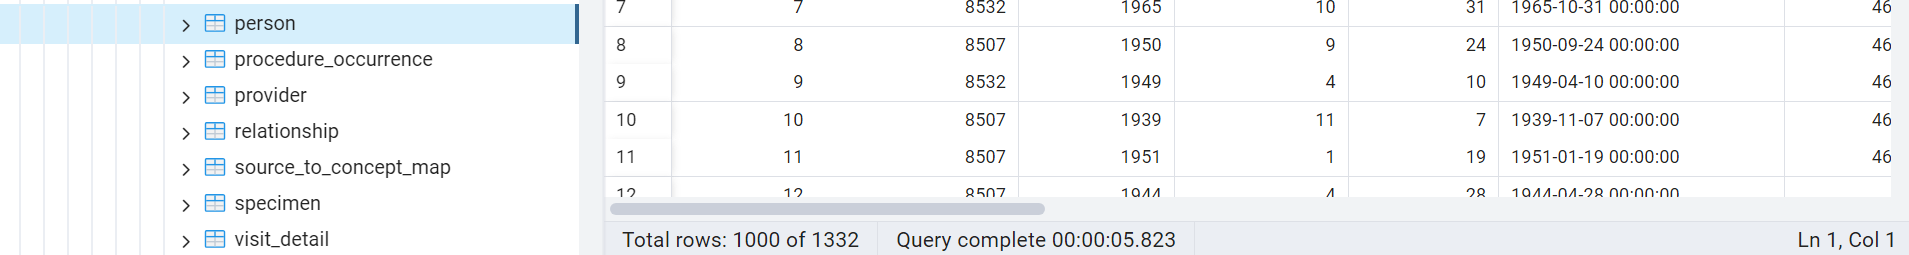
\includegraphics[width=0.90\textwidth]{figures/personCount.png}
    \caption{Captura de pantalla de pgAdmin del número de instancias de la tabla \code{person}}
    \label{figure:personCount}
\end{figure}

\begin{figure}[H]
    \centering
    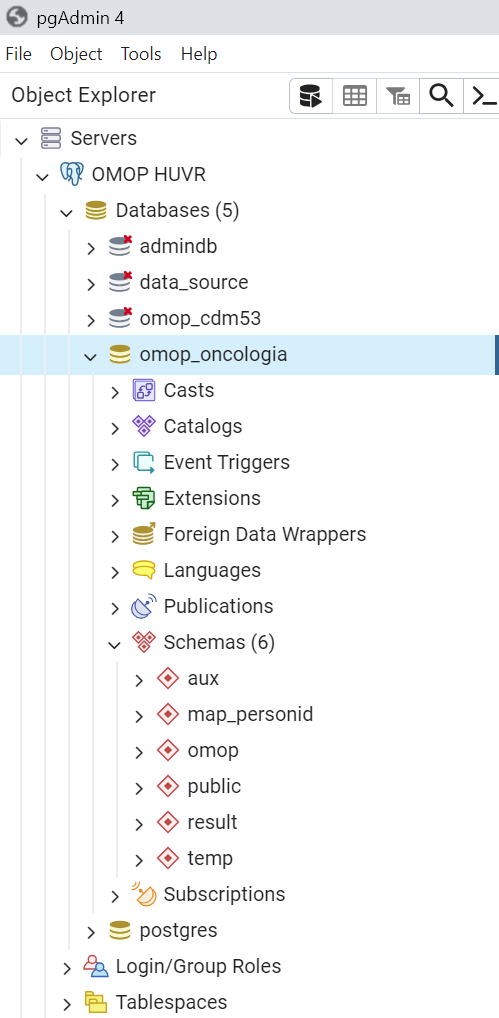
\includegraphics[width=0.50\textwidth]{figures/servidorHUVR.png}
    \caption{Captura de pantalla de pgAdmin de la estructura del servidor del HUVR}
    \label{figure:servidorHUVR}
\end{figure}


\section{Integración de la BD en ATLAS Broadsea}

El proceso de integración de una base de datos externa en la WebAPI de Broadsea se describe con gran detalle en el Anexo \ref{anexo:manual} ''Manual de instalación, despliegue y configuración de ATLAS Broadsea''. No obstante, en esta subsección se presenta de forma sencilla el proceso de conexión con la base de datos del HUVR.

Para establecer la conexión con una base de datos externa se debe registrar la base de datos en el esquema de la WebAPI de Broadsea, concretamente en las tablas \code{source} y \code{source\_daimon}. Para ello se ejecuta un conjunto de queries disponibles en el archivo del repositorio de github \code{Thesis-ATLAS-OHDSI/files/thesis/sql/queries\_insert\_huvr\_source.sql}. 

En las Figuras \ref{figure:sourceHUVR} ''Captura de pantalla de pgAdmin de la tabla \code{source}'' y \ref{figure:source_daimonHUVR} ''Captura de pantalla de pgAdmin de la tabla \code{source\_daimon}'' se muestran los resultados de la ejecución correcta de las queries. 

\begin{figure}[H]
    \centering
    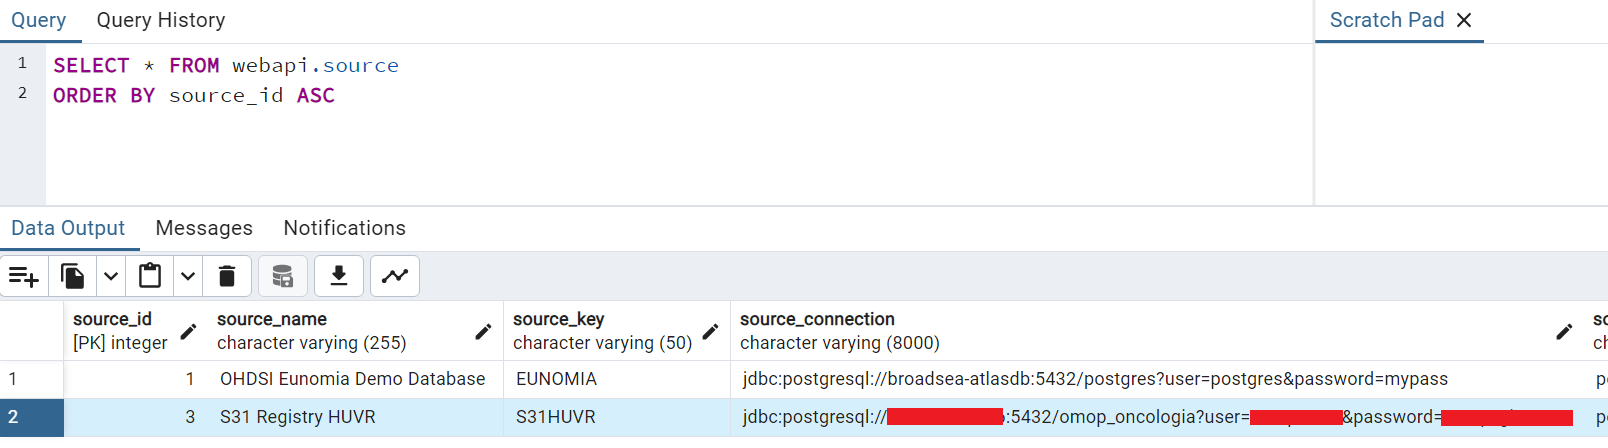
\includegraphics[width=0.90\textwidth]{figures/sourceHUVR.png}
    \caption{Captura de pantalla de pgAdmin de la tabla \code{source}}
    \label{figure:sourceHUVR}
\end{figure}

\begin{figure}[H]
    \centering
    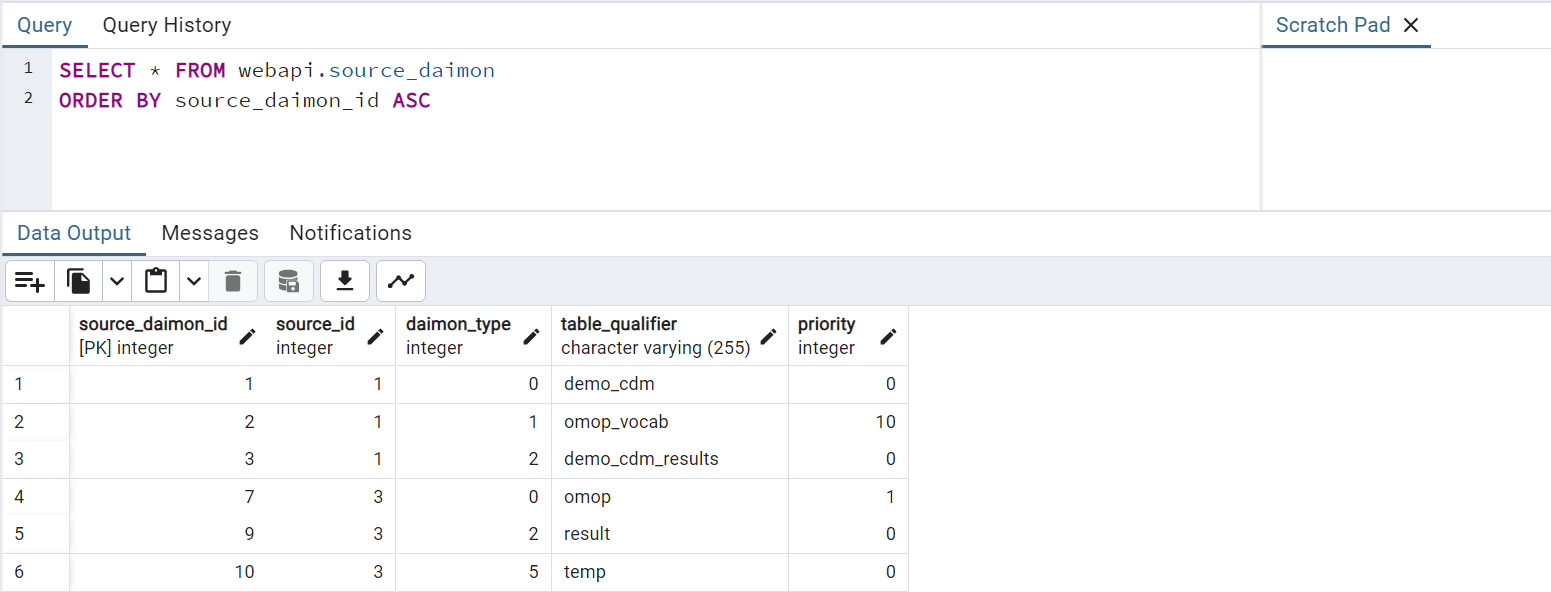
\includegraphics[width=0.75\textwidth]{figures/source_daimonHUVR.png}
    \caption{Captura de pantalla de pgAdmin de la tabla \code{source\_daimon}}
    \label{figure:source_daimonHUVR}
\end{figure}

Se puede comprobar que la integración de la base de datos en Broadsea se ha realizado correctamente a través del menú \code{configuration} de ATLAS, donde se muestran los detalles de las bases de datos integradas con la herramienta. En la Figura \ref{figure:configATLAS} ''Captura de pantalla de menú \code{configuration} de ATLAS Broadsea'' se observa que hay dos bases de datos: la base de datos de Eunomia que viene preinstalada con Broadsea y la base de datos recién instalada.

\begin{figure}[H]
    \centering
    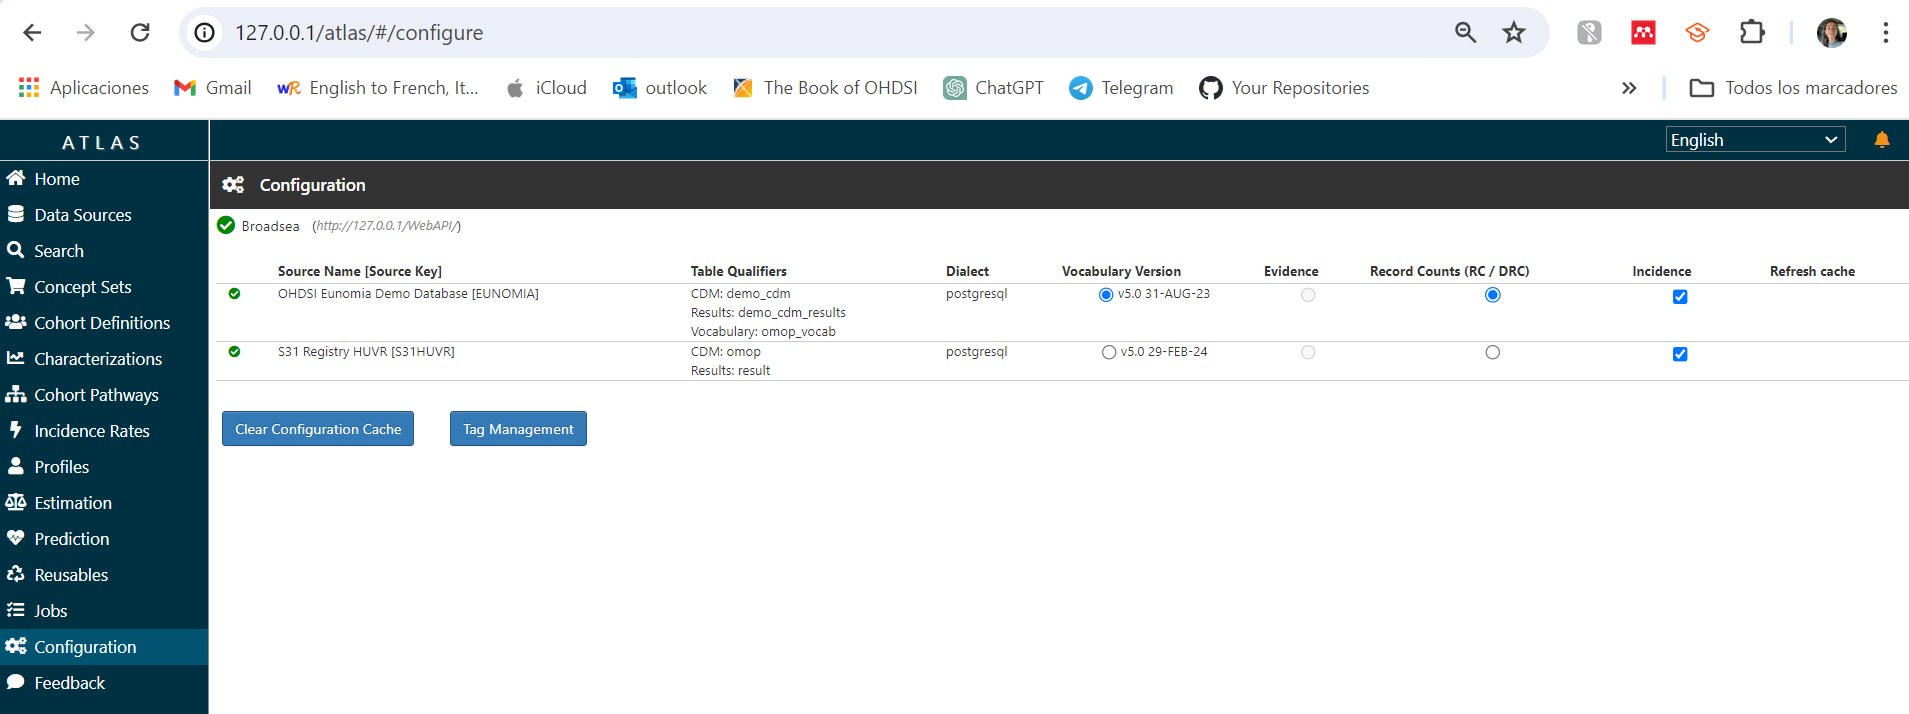
\includegraphics[width=0.90\textwidth]{figures/configATLAS.png}
    \caption{Captura de pantalla de menú \code{configuration} de ATLAS Broadsea}
    \label{figure:configATLAS}
\end{figure}
    \chapter{Reportes de la BD} \label{cap:03reporte}

La obtención de un reporte de la base de datos utilizando ATLAS es un proceso muy sencillo. Accediendo al menú lateral \code{Data Sources} se abre una interfaz que permite seleccionar la base de datos de la que se quiere obtener el reporte y el tipo de reporte que se quiere obtener.

\begin{figure}[H]
    \centering
    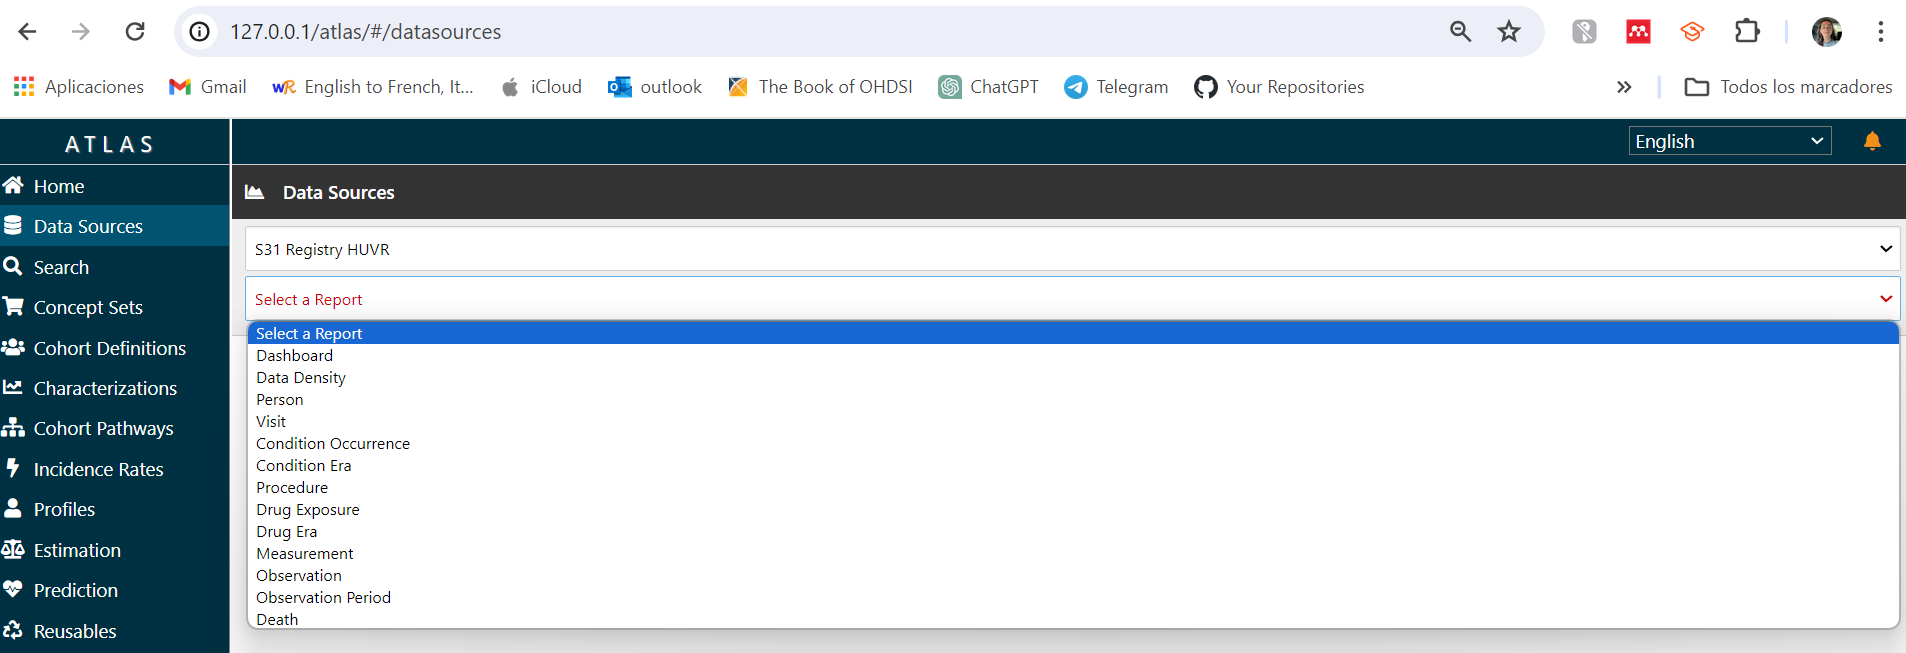
\includegraphics[width=1\textwidth]{figures/atlasDataSources.png}
    \caption{Captura de pantalla de la interfaz principal del menú \code{Data Sources}}
    \label{figure:atlasDataSources}
\end{figure}

A continuación se generan algunos reportes para realizar un análisis exploratorio de la base de datos. Todas las imágenes que se obtienen en cada reporte se encuentran en el repositorio de github \code{Thesis-ATLAS-OHDSI/atlas}.

\begin{figure}[H]
    \centering
    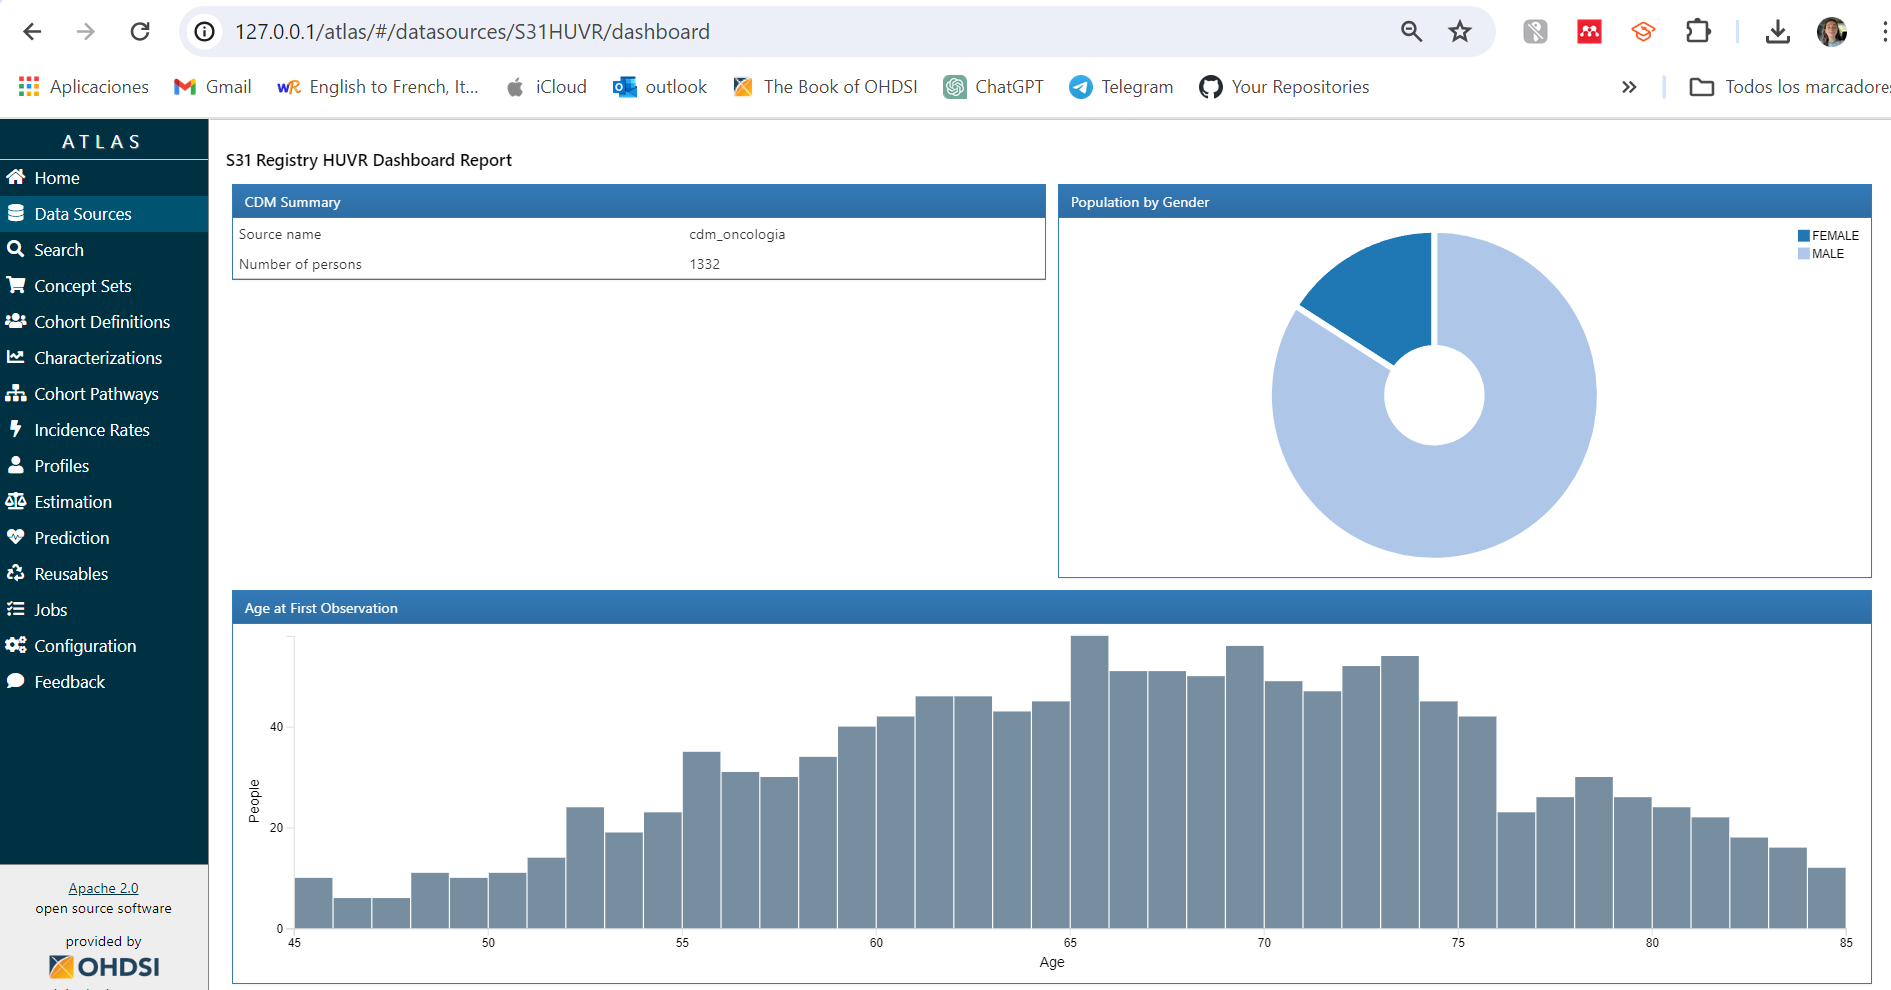
\includegraphics[width=1\textwidth]{figures/atlasCAPdashboard.png}
    \caption{Captura de pantalla del reporte \code{Dashboard} generado en ATLAS Broadsea}
    \label{figure:atlasCAPdashboard}
\end{figure}

\begin{figure}[H]
    \centering
    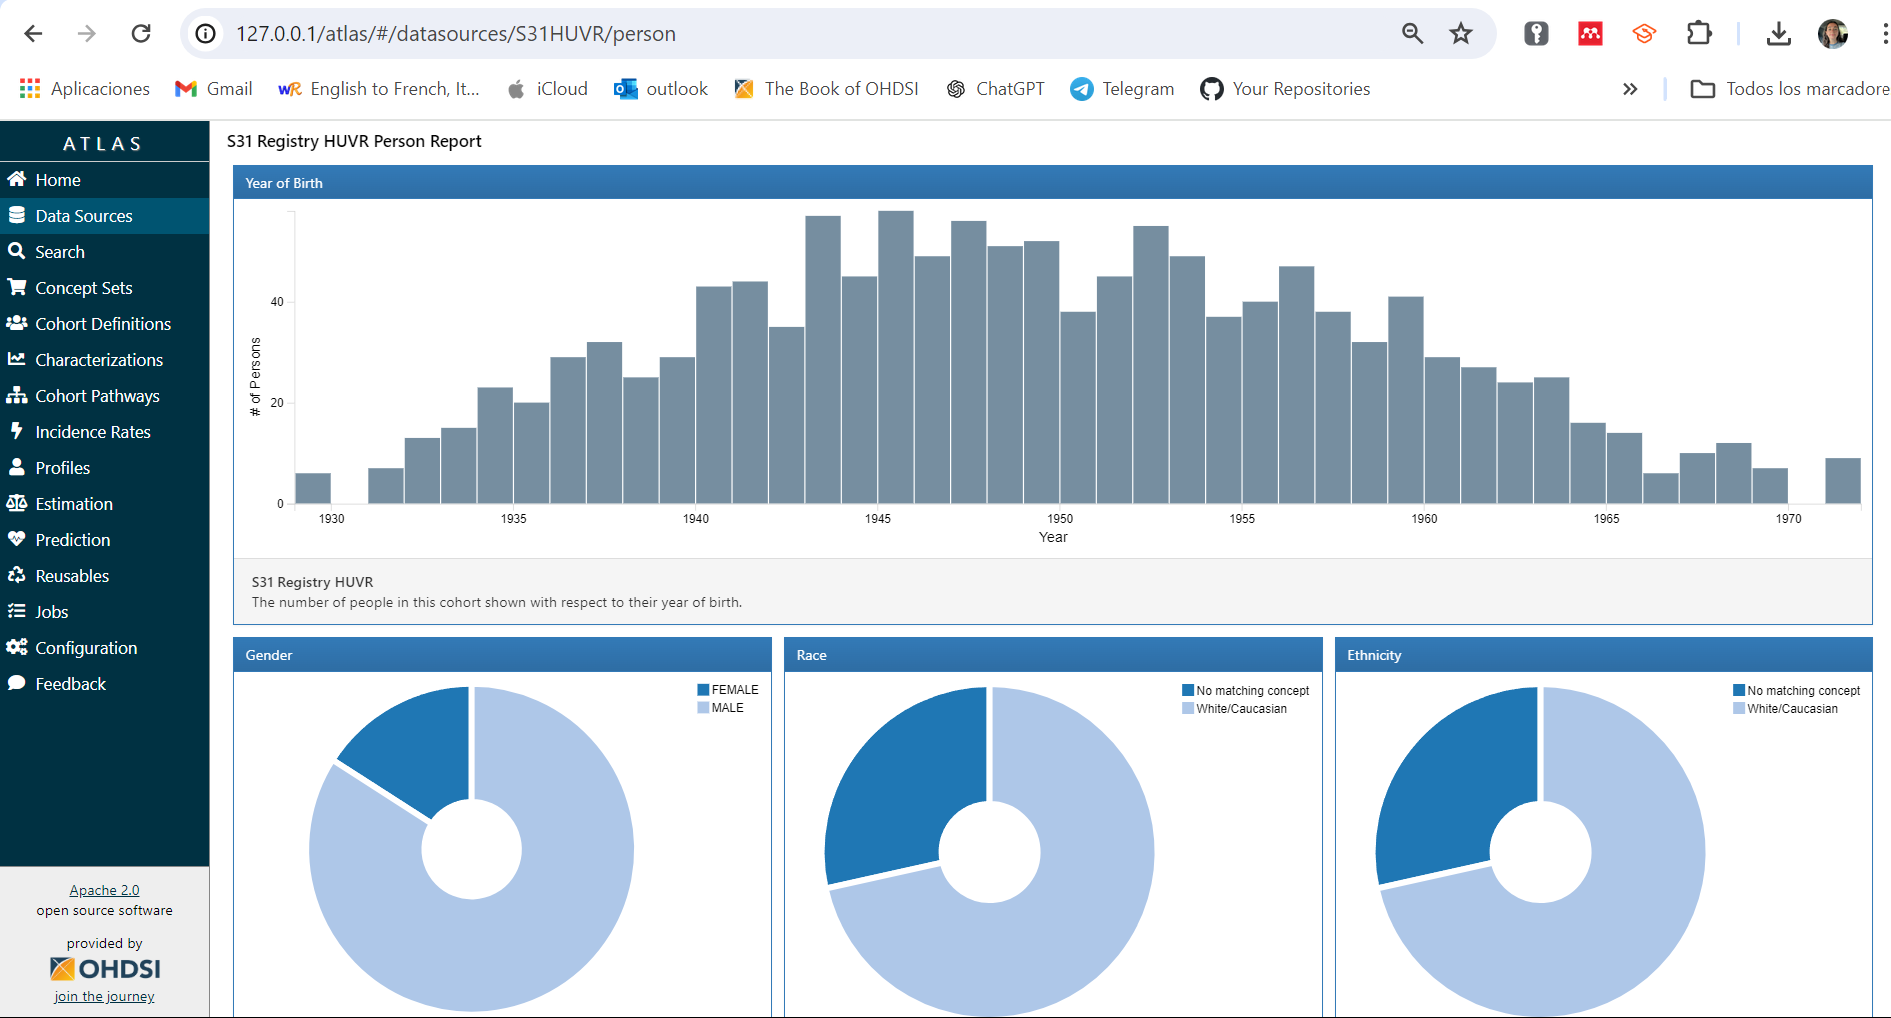
\includegraphics[width=1\textwidth]{figures/atlasREPORTperson.png}
    \caption{Captura de pantalla del reporte \code{Person} generado en ATLAS Broadsea}
    \label{figure:atlasREPORTperson}
\end{figure}

\begin{figure}[H]
    \centering
    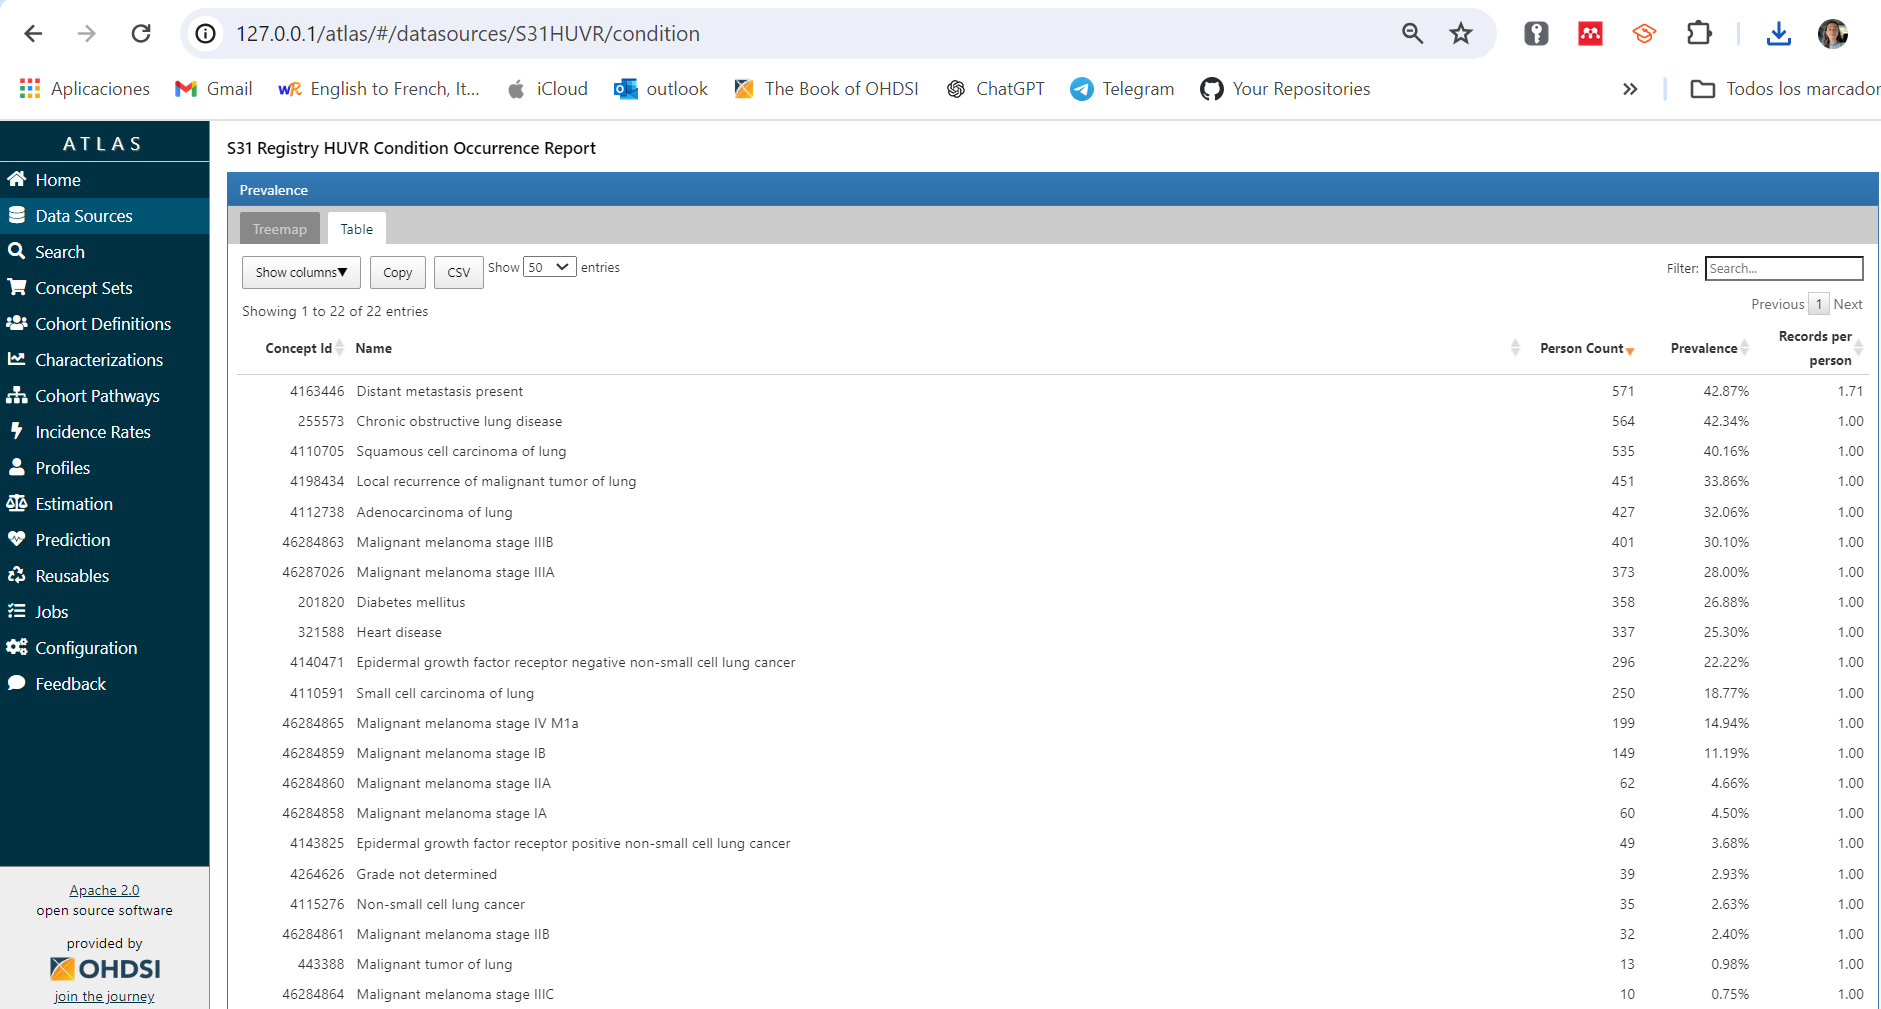
\includegraphics[width=1\textwidth]{figures/atlasREPORTcondition_ocurrence.png}
    \caption{Captura de pantalla del reporte \code{Condition Ocurrence} generado en ATLAS Broadsea}
    \label{figure:atlasREPORTcondition_ocurrence}
\end{figure}

\begin{figure}[H]
    \centering
    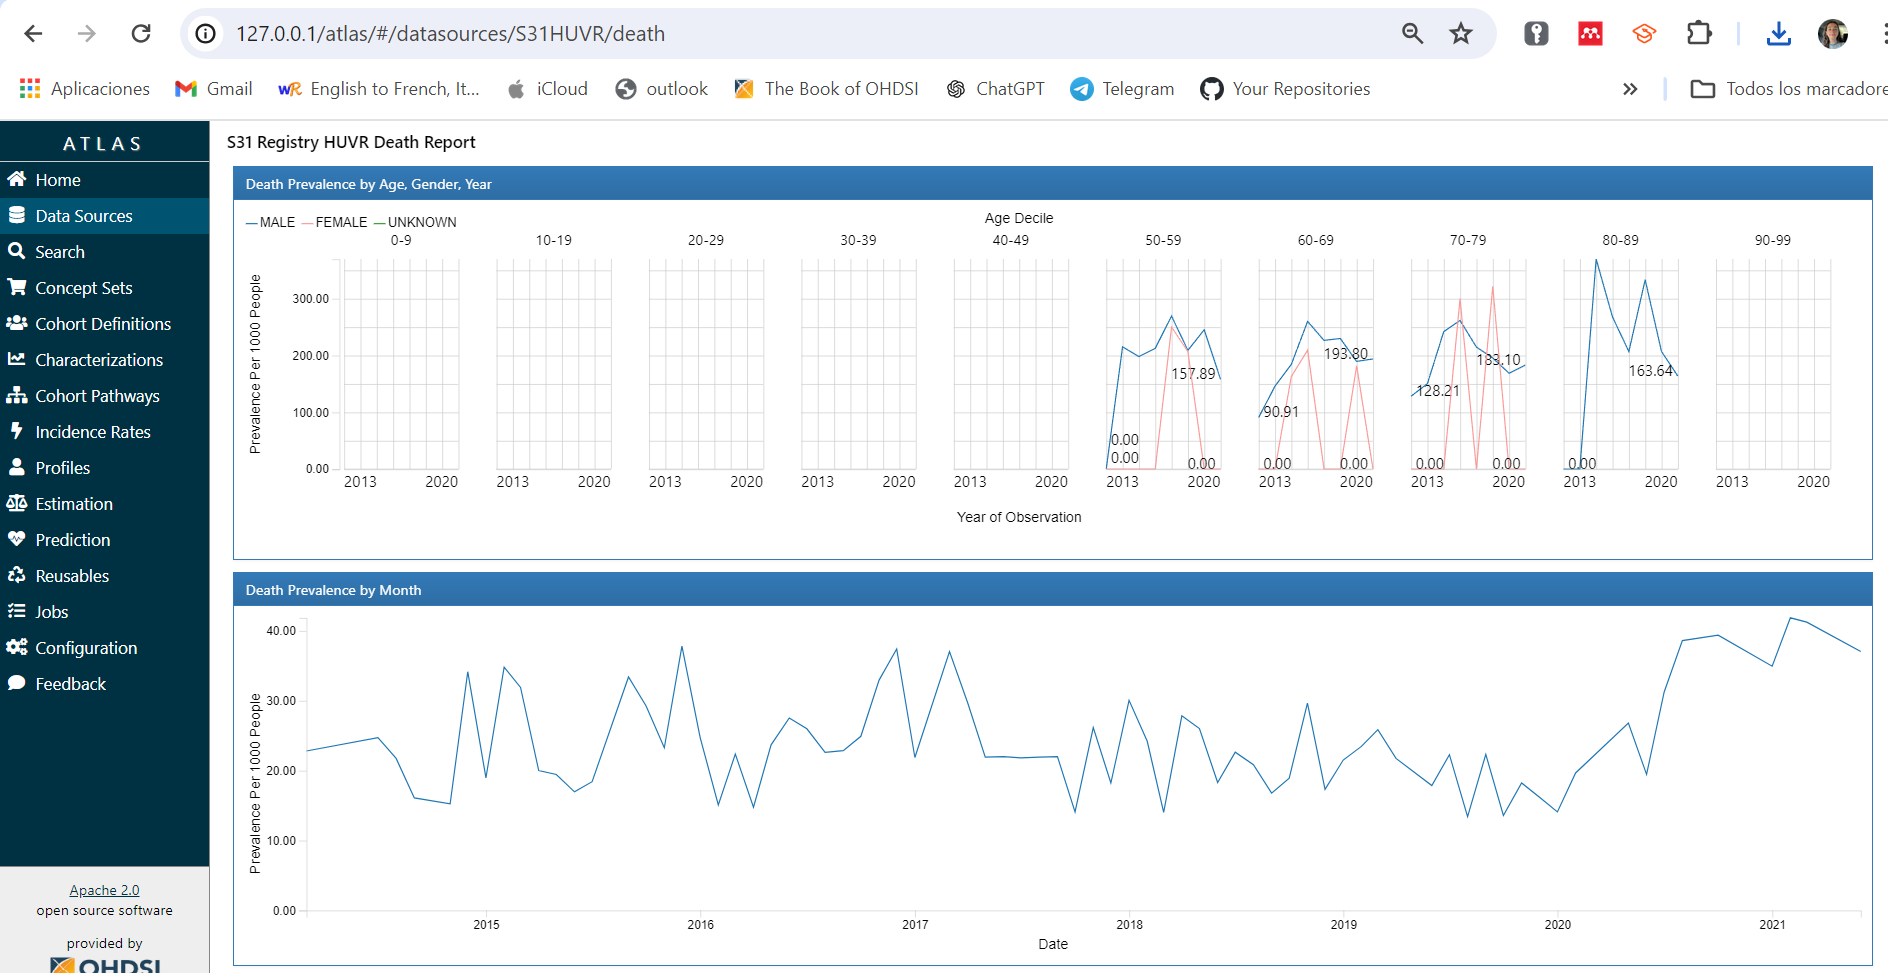
\includegraphics[width=1\textwidth]{figures/atlasREPORTdeath.png}
    \caption{Captura de pantalla del reporte \code{Death} generado en ATLAS Broadsea}
    \label{figure:atlasREPORTdeath}
\end{figure}

\begin{figure}[H]
    \centering
    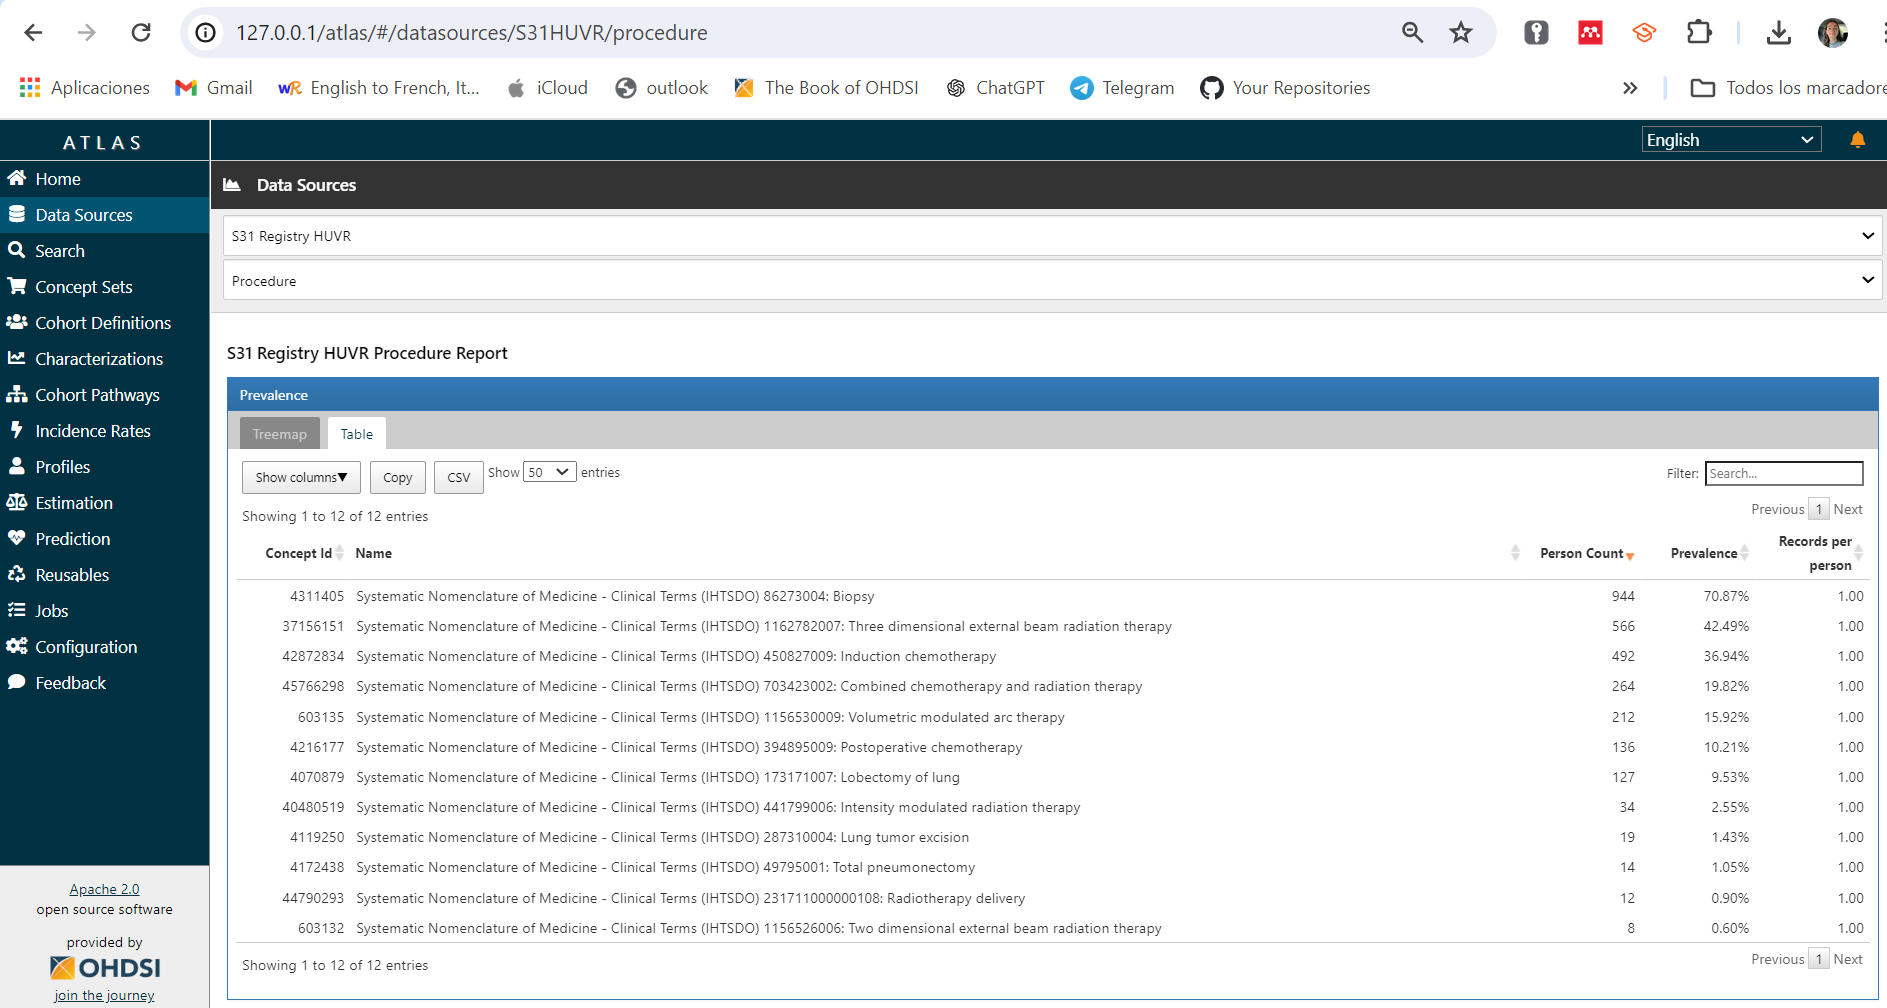
\includegraphics[width=1\textwidth]{figures/atlasREPORTprocedure.png}
    \caption{Captura de pantalla del reporte \code{Procedure} generado en ATLAS Broadsea}
    \label{figure:atlasREPORTprocedure}
\end{figure}

\begin{figure}[H]
    \centering
    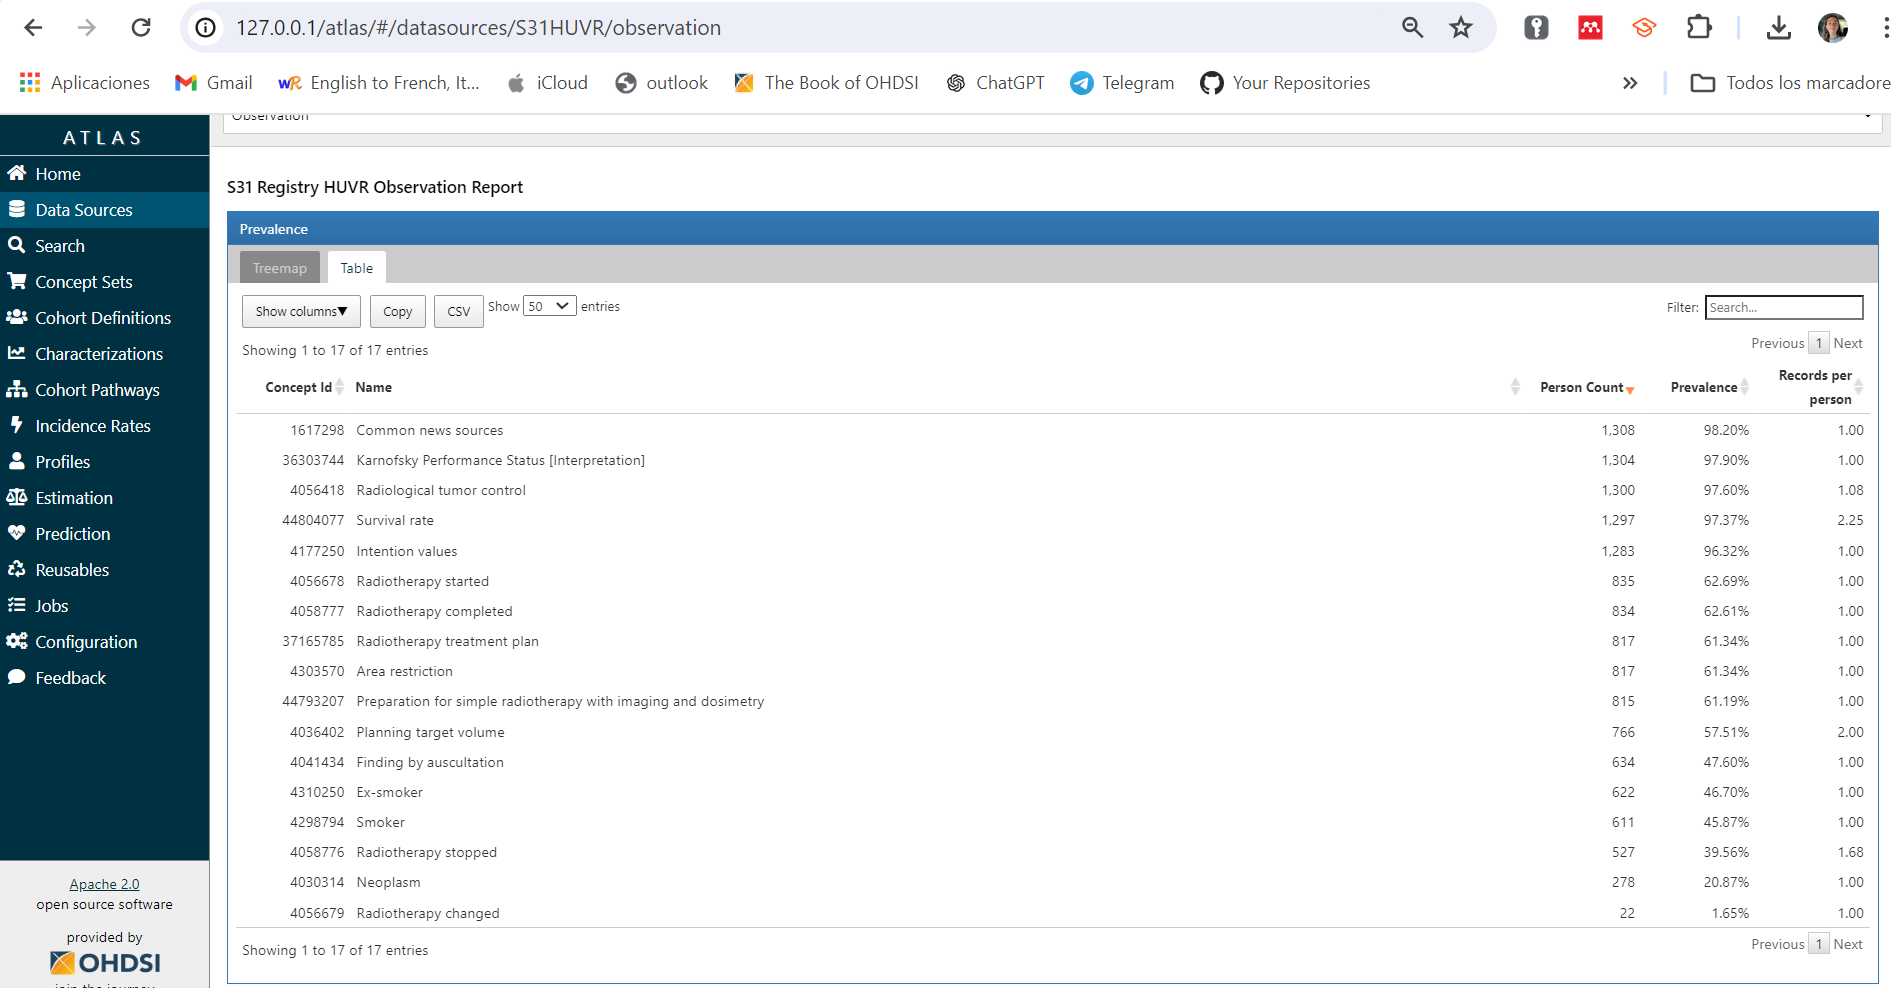
\includegraphics[width=1\textwidth]{figures/atlasREPORTobservation.png}
    \caption{Captura de pantalla del reporte \code{Observation} generado en ATLAS Broadsea}
    \label{figure:atlasREPORTobservation}
\end{figure}
    \chapter{Definición de grupos de conceptos} \label{cap:04concepto}

Para definir los grupos de conceptos es muy importante realizar la  exploración previa de las condiciones, observaciones y procedimientos  en los reportes de la base de datos (véase la sección anterior \ref{cap:03reporte} ''Reportes de la BD'').

Como en este caso, el análisis solo utiliza una fuente de datos, la base de datos S31 Registry HUVR, en la mayoría de los casos la definición de los grupos de conceptos incluye específicamente solamente los conceptos que intervienen en esta base de datos. Para estandarizar estos grupos de conceptos a cualquier base de datos y realizar el análisis en varias fuentes diferentes a la vez, bastaría con incluir también todos los descendientes de cada concepto incluído. Gracias a esta funcionalidad de ATLAS, un grupo de conceptos muy específico puede extenderse en un grupo mucho más vasto y genérico.

Por tanto, para definir los grupos de conceptos se ha seguido el siguiente procedimiento:

\begin{enumerate}
    \item \textbf{Obtener ID de los términos concretos.} Dado que un mismo concepto clínico puede expresarse con diferentes terminologías, el objetivo de esta primera tarea es identificar exactamente los términos que utiliza la base de datos.

    Para ello, se puede consultar los conceptos la base de datos directamente a través del administrador de la base de datos o se pueden visualizar a través de la herramienta \code{Data Sources} de ATLAS.

    \begin{enumerate}[label=\alph*.]
        \item \textbf{A través de pgAdmin.} Para ello ejecutamos \textit{queries} sobre la BD que devuelvan los identificadores únicos de las observaciones, condiciones y procedimientos registrados en la base de datos. Estas queries se encuentran disponibles en el repositorio de github del proyecto, en la ruta \code{Thesis-ATLAS-OHDSI/files/thesis/sql/omop\_s31\_exploration.sql}. A continuación se muestra un extracto del código.

\begin{lstlisting}[language=sql]
-- Obtiene las distintas enfermedades registradas en la BD
SELECT DISTINCT condition_concept_id FROM omop.condition_occurrence

-- Obtiene las distintas observaciones registradas en la BD
SELECT DISTINCT observation_concept_id FROM omop.observation

-- Obtiene los distintos procedimientos registrados en la BD
SELECT DISTINCT procedure_concept_id FROM omop.procedure_occurrence
\end{lstlisting}


        \item \textbf{A través de Data Source.} Para ello basta con generar los reportes de \code{Condition Ocurrence}, \code{Observation} y \code{Procedure}, tal como se realiza en la sección anterior en las Figuras \ref{figure:atlasREPORTcondition_ocurrence}, \ref{figure:atlasREPORTobservation}, \ref{figure:atlasREPORTprocedure}.
        
    \end{enumerate}

    \item \textbf{Definir un nuevo grupo de conceptos.} Una vez se conoce los términos específicos que utiliza la base de datos para nombrar los conceptos clínicos, se utiliza la herramienta \code{Concept Sets} de ATLAS para definir un nuevo grupo de concepto para cada concepto clínico en general. 

    Para la realización de este estudio se han definido 12 grupos de conceptos, tal y como muestra la Figura \ref{figure:conceptSetsCAP} ''Listado de grupos de conceptos definidos''.

\begin{figure}[H]
    \centering
    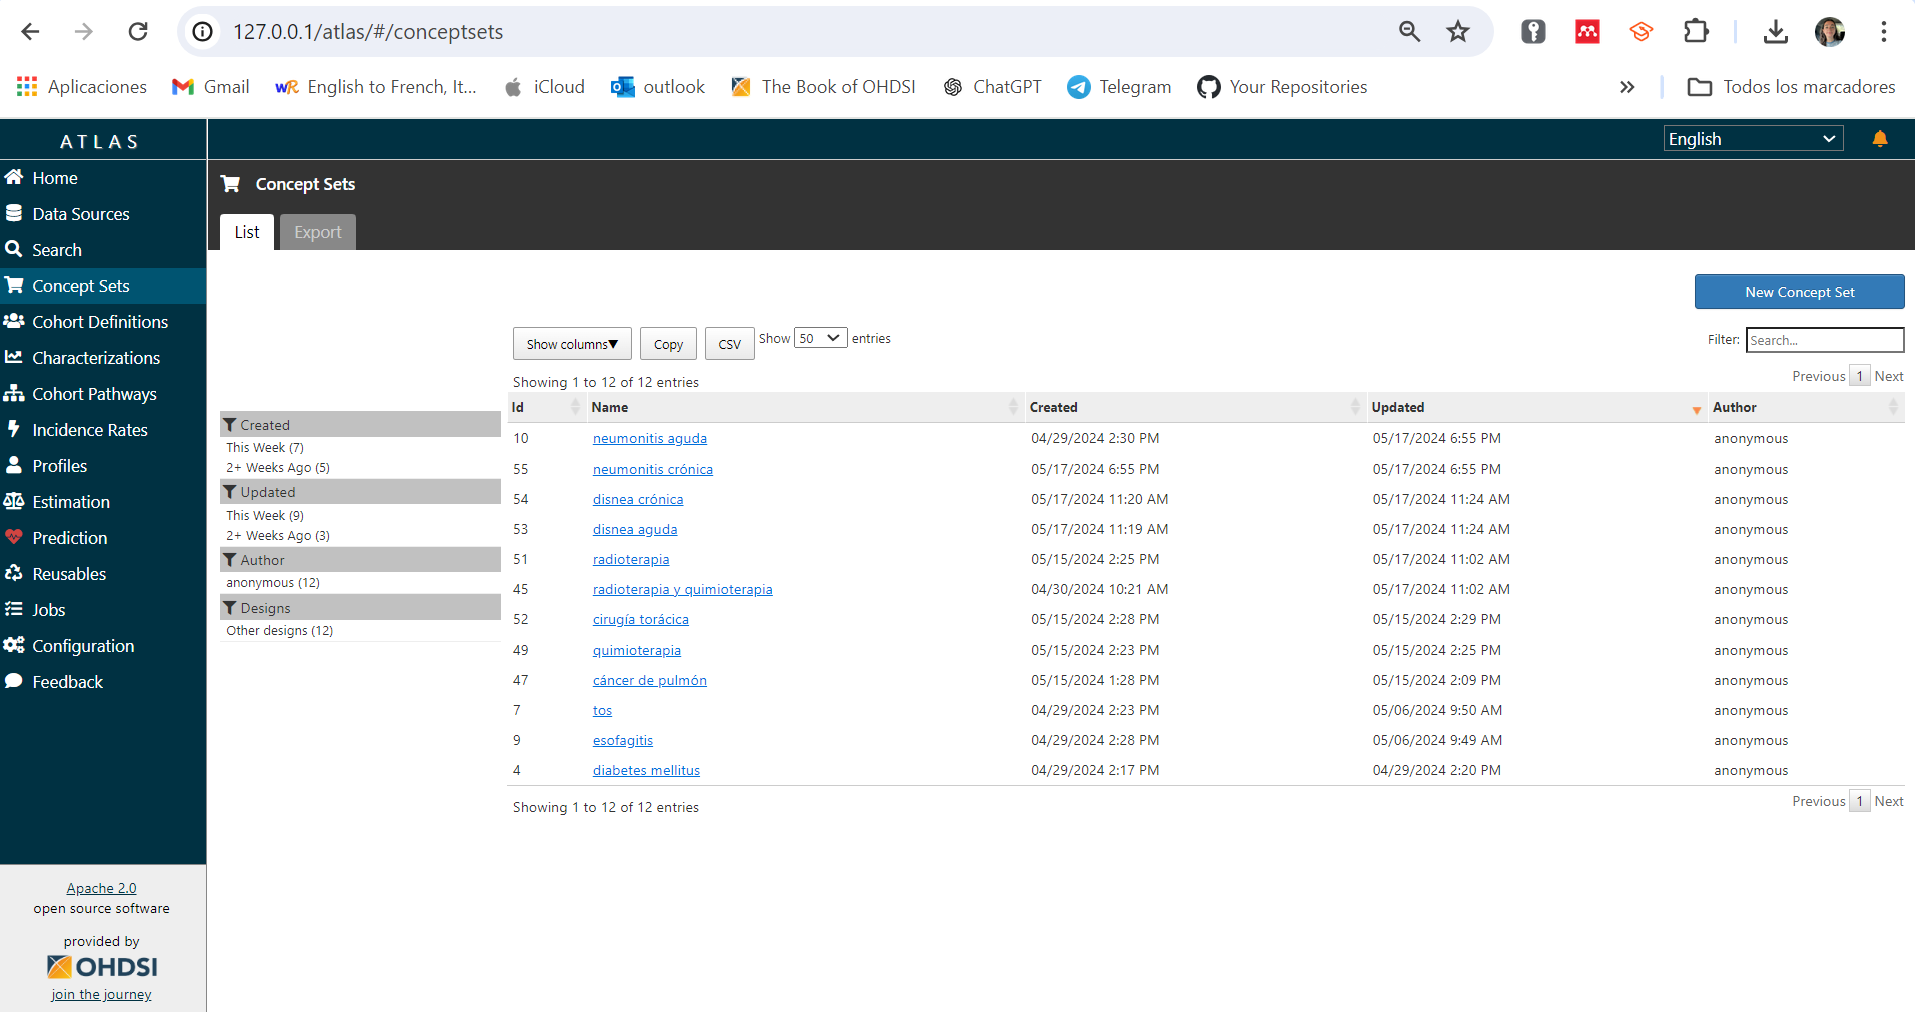
\includegraphics[width=0.90\textwidth]{figures/conceptSetsCAP.png}
    \caption{Listado de grupos de conceptos definidos}
    \label{figure:conceptSetsCAP}
\end{figure}

    \item \textbf{Exportar un grupo de conceptos.} Una vez definidos los grupos de conceptos estos se pueden exportar a formato \textbf{json} para favorecer el intercambio de información entre sistemas o la reutilización en otros estudios. ATLAS permite definir nuevos grupos de conceptos o importarlos de un archivo json, favoreciendo también la reproducibilidad del estudio. 

    A continuacións se muestra un ejemplo del formato que presentan estos conceptos una vez exportados a json.
    
\begin{lstlisting}[language=json]
{
    "ConceptSets": [
      {
        "id": 0,
        "name": "neumonitis crónica",
        "expression": {
          "items": [
            {
              "concept": {
                "CONCEPT_CLASS_ID": "Clinical Finding",
                "CONCEPT_CODE": "405569006",
                "CONCEPT_ID": 4226132,
                "CONCEPT_NAME": "Post-radiotherapy pneumonitis",
                "DOMAIN_ID": "Condition",
                "INVALID_REASON": "V",
                "INVALID_REASON_CAPTION": "Valid",
                "STANDARD_CONCEPT": "S",
                "STANDARD_CONCEPT_CAPTION": "Standard",
                "VOCABULARY_ID": "SNOMED"
              },
              "includeDescendants": true
            }
          ]
        }
      }
    ],
    "PrimaryCriteria": {
      "CriteriaList": [
        {
          "ConditionOccurrence": {
            "CodesetId": 0
          }
        }
      ],
      "ObservationWindow": {
        "PriorDays": 0,
        "PostDays": 0
      },
      "PrimaryCriteriaLimit": {
        "Type": "First"
      }
    },
    "QualifiedLimit": {
      "Type": "First"
    },
    "ExpressionLimit": {
      "Type": "First"
    },
    "InclusionRules": [],
    "CensoringCriteria": [],
    "CollapseSettings": {
      "CollapseType": "ERA",
      "EraPad": 0
    },
    "CensorWindow": {},
    "cdmVersionRange": ">=5.0.0"
  }
\end{lstlisting}


    Todos los conceptos utilizados en el proyecto se han exportado a formato json y almacenado en el repositorio de github en la ruta \code{Thesis-ATLAS-OHDSI/atlas/concept sets} para que sean accesibles públicamente.
    
\end{enumerate}
    \chapter{Definición de cohortes} \label{cap:05cohortes}

Las cohortes se definen en NB FINALFINALCLEANNEWDATA


- TARGET COHORT

- OUTCOME COHORT
    \chapter{Caracterización} \label{cap:06caracterizacion}

- NIVEL ESTADISTICO

- COHORT PATHWAY
    \chapter{Estimación a Nivel de Población} \label{cap:08PLE}


    \chapter{Predicción a Nivel de Paciente} \label{cap:08PLP}

- TRIPOD AI


    \bibliographystyle{unsrtnat}
    \bibliography{bibliografia.bib}

        

% Fin del documento
\end{document}
